\documentclass[answers]{exam}
\usepackage[english,spanish]{babel}
\usepackage[utf8]{inputenc}
\usepackage{amsmath, amssymb}
\usepackage{graphicx}
\usepackage{enumitem}

\begin{document}

\begin{questions}

    \question Escriba solo si la proposición es verdadera o falsa.

    \begin{minipage}{\textwidth}
        \centering
        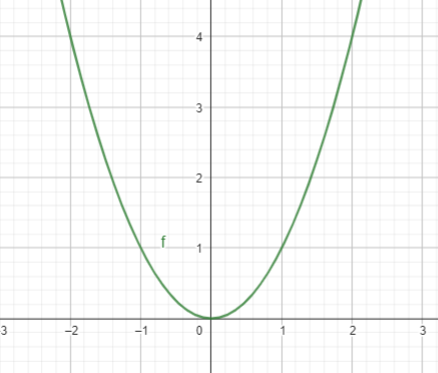
\includegraphics[width=0.3\textwidth]{public/image.png}\\
    \end{minipage}

    \begin{parts}
        \part El principio de Inducción matemática es un método que permite verificar enunciados matemáticos.
        \part Se puede aplicar el determinante de una matriz a cualquier sistema de ecuaciones.
        \part La matriz escalonada reducida no tiene solución.
        \[
        \begin{bmatrix}
        1 & 1 & 0 & 0 & 0 & -5\\
        2 & 0 & 0 & 1 & 0 & 4\\
        3 & 0 & 0 & 0 & 1 & -5\\
        4 & 0 & 0 & 0 & 0 & 0
        \end{bmatrix}
        \]
        \part Puede \((3,-1,4)\) ser escrito como combinación lineal de \((1,-1,0)\), \((0,1,1)\) y \((3,-5,-2)\).
        \part ¿El conjunto \(S = \{(0,0,1), (0,1,0), (1,0,0)\}\) es un conjunto de vectores linealmente independientes?
    \end{parts}

    \begin{solution}
        \begin{parts}
            \part Verdadero. 
            \part Falso. 
            \part Falso.
            \[
            \begin{bmatrix}
            0 & 1 & 0 & 0 & 0 & -5\\
            0 & 0 & 0 & 1 & 0 & 4\\
            0 & 0 & 0 & 0 & 1 & -5\\
            0 & 0 & 0 & 0 & 0 & 0
            \end{bmatrix}
            \]
            \part Falso.
            \part Falso.
        \end{parts}
        \end{solution}
                

    \question Use la sustitución hacia atrás para resolver el sistema de ecuaciones. Escriba así \((x,y,z)\) la solución.

    \[
    \begin{aligned}
    2x - y + 5z &= 24 \\
    y + 2z &= 6 \\
    z &= 8
    \end{aligned}
    \]

    \begin{solution}
        \[
        z = 8
        \]
        \[
        y + 2(8) = 6 \quad \Rightarrow \quad y = -10
        \]
        \[
        2x - (-10) + 5(8) = 24 \quad \Rightarrow \quad x = -13
        \]
        
        Solución: \((-13, -10, 8)\)
        \end{solution}
        

    \question Encontrar una matriz \(X\) tal que 

    \[
    \begin{bmatrix}
    1 & 0 & 0\\
    4 & 1 & 0\\
    0 & 4 & 1\\
    \end{bmatrix} 
    X = 
    \begin{bmatrix}
    1 & 0\\
    0 & 1\\
    1 & 1\\
    \end{bmatrix}
    \]

    \begin{solution}
        Queremos encontrar una matriz \( X \) tal que:
        
        \[
        \begin{bmatrix}
         1 & 0 & 0\\
         4 & 1 & 0\\
         0 & 4 & 1
        \end{bmatrix} 
        X = 
        \begin{bmatrix}
         1 & 0\\
         0 & 1\\
         1 & 1
        \end{bmatrix}
        \]
        
        Sea \( X = \begin{bmatrix}
         x_{11} & x_{12} \\
         x_{21} & x_{22} \\
         x_{31} & x_{32}
        \end{bmatrix} \). Multiplicamos:
        
        \[
        \begin{bmatrix}
         1 & 0 & 0\\
         4 & 1 & 0\\
         0 & 4 & 1
        \end{bmatrix} 
        \begin{bmatrix}
         x_{11} & x_{12} \\
         x_{21} & x_{22} \\
         x_{31} & x_{32}
        \end{bmatrix} 
        =
        \begin{bmatrix}
         1 \cdot x_{11} + 0 \cdot x_{21} + 0 \cdot x_{31} & 1 \cdot x_{12} + 0 \cdot x_{22} + 0 \cdot x_{32} \\
         4 \cdot x_{11} + 1 \cdot x_{21} + 0 \cdot x_{31} & 4 \cdot x_{12} + 1 \cdot x_{22} + 0 \cdot x_{32} \\
         0 \cdot x_{11} + 4 \cdot x_{21} + 1 \cdot x_{31} & 0 \cdot x_{12} + 4 \cdot x_{22} + 1 \cdot x_{32}
        \end{bmatrix}
        \]
        
        Igualando a la matriz objetivo:
        
        \[
        \begin{bmatrix}
         x_{11} & x_{12} \\
         4x_{11} + x_{21} & 4x_{12} + x_{22} \\
         4x_{21} + x_{31} & 4x_{22} + x_{32}
        \end{bmatrix} 
        =
        \begin{bmatrix}
         1 & 0 \\
         0 & 1 \\
         1 & 1
        \end{bmatrix}
        \]
        
        De aquí obtenemos el sistema de ecuaciones:
        
        \[
        \begin{aligned}
        x_{11} &= 1 \\
        x_{12} &= 0 \\
        4x_{11} + x_{21} &= 0 \Rightarrow x_{21} = -4 \\
        4x_{12} + x_{22} &= 1 \Rightarrow x_{22} = 1 \\
        4x_{21} + x_{31} &= 1 \Rightarrow x_{31} = 1 \\
        4x_{22} + x_{32} &= 1 \Rightarrow x_{32} = 1
        \end{aligned}
        \]
        
        Por lo tanto, la matriz \( X \) es:
        
        \[
        X = 
        \begin{bmatrix}
         1 & 0 \\
         -4 & 1 \\
         1 & 1
        \end{bmatrix}
        \]
        \end{solution}
        
        
    
    \question Determine el tipo de solución y cuántas variables libres para el siguiente sistema de ecuaciones.

    \[
    \begin{aligned}
    x - 2y + 5z &= 2 \\
    3x - 6y + 15z &= 0
    \end{aligned}
    \]

    \begin{solution}
        El sistema de ecuaciones es:
        
        \[
        \begin{aligned}
        x - 2y + 5z &= 2 \\
        3x - 6y + 15z &= 0
        \end{aligned}
        \]
        
        Representamos el sistema en forma de matriz aumentada:
        
        \[
        \left[\begin{array}{ccc|c}
        1 & -2 & 5 & 2 \\
        3 & -6 & 15 & 0
        \end{array}\right]
        \]
        
        Realizamos la reducción de Gauss-Jordan:
        
        1. **Paso 1:** Sustituir la fila 2 por la fila 2 menos 3 veces la fila 1.
        
        \[
        \left[\begin{array}{ccc|c}
        1 & -2 & 5 & 2 \\
        0 & 0 & 0 & -6
        \end{array}\right]
        \]
        
        2. **Paso 2:** La fila 2 muestra que \(0 = -6\), que es una contradicción.
        
        \textbf{Conclusión:} El sistema es inconsistente y no tiene solución. 
        \end{solution}
        
        

    \question Demostrar la siguiente expresión matemática por inducción matemática.

    \[
        \frac{1}{1 \cdot 4} + \frac{1}{4 \cdot 7} + \frac{1}{7 \cdot 10} + \ldots + \frac{1}{(3n-2)\cdot(3n+1)} = \frac{n}{3n+1}
    \]
    \begin{solution}
        \textbf{Demostración por inducción:}
        
        1. **Base de inducción:**
        
        Para \(n = 1\):
        \[
        \frac{1}{1 \cdot 4} = \frac{1}{4} \quad \text{y} \quad \frac{1}{3 \cdot 1 + 1} = \frac{1}{4}
        \]
        La base es verdadera.
        
        2. **Paso inductivo:**
        
        Supongamos que la fórmula es cierta para \(n = k\):
        \[
        \frac{1}{1 \cdot 4} + \frac{1}{4 \cdot 7} + \dots + \frac{1}{(3k-2)\cdot(3k+1)} = \frac{k}{3k+1}
        \]
        Demuéstralo para \(n = k+1\):
        
        \[
        \text{Añade el término } \frac{1}{(3(k+1)-2)\cdot(3(k+1)+1)} = \frac{1}{(3k+1)(3k+4)}
        \]
        \[
        \frac{k}{3k+1} + \frac{1}{(3k+1)(3k+4)} = \frac{k(3k+4) + 1}{(3k+1)(3k+4)} = \frac{3k^2 + 4k + 1}{(3k+1)(3k+4)}
        \]
        \[
        \text{Factoriza:} \quad \frac{(k+1)(3k+1)}{(3k+1)(3k+4)} = \frac{k+1}{3(k+1) + 1}
        \]
        \[
        \text{Por lo tanto, la fórmula es verdadera para } n = k+1.
        \]
        \textbf{Conclusión:} La fórmula es verdadera para todo \(n \geq 1\) por inducción matemática.
        \end{solution}
        
\end{questions}

\end{document}
